\documentclass[1p]{elsarticle_modified}
%\bibliographystyle{elsarticle-num}

%\usepackage[colorlinks]{hyperref}
%\usepackage{abbrmath_seonhwa} %\Abb, \Ascr, \Acal ,\Abf, \Afrak
\usepackage{amsfonts}
\usepackage{amssymb}
\usepackage{amsmath}
\usepackage{amsthm}
\usepackage{scalefnt}
\usepackage{amsbsy}
\usepackage{kotex}
\usepackage{caption}
\usepackage{subfig}
\usepackage{color}
\usepackage{graphicx}
\usepackage{xcolor} %% white, black, red, green, blue, cyan, magenta, yellow
\usepackage{float}
\usepackage{setspace}
\usepackage{hyperref}

\usepackage{tikz}
\usetikzlibrary{arrows}

\usepackage{multirow}
\usepackage{array} % fixed length table
\usepackage{hhline}

%%%%%%%%%%%%%%%%%%%%%
\makeatletter
\renewcommand*\env@matrix[1][\arraystretch]{%
	\edef\arraystretch{#1}%
	\hskip -\arraycolsep
	\let\@ifnextchar\new@ifnextchar
	\array{*\c@MaxMatrixCols c}}
\makeatother %https://tex.stackexchange.com/questions/14071/how-can-i-increase-the-line-spacing-in-a-matrix
%%%%%%%%%%%%%%%

\usepackage[normalem]{ulem}

\newcommand{\msout}[1]{\ifmmode\text{\sout{\ensuremath{#1}}}\else\sout{#1}\fi}
%SOURCE: \msout is \stkout macro in https://tex.stackexchange.com/questions/20609/strikeout-in-math-mode

\newcommand{\cancel}[1]{
	\ifmmode
	{\color{red}\msout{#1}}
	\else
	{\color{red}\sout{#1}}
	\fi
}

\newcommand{\add}[1]{
	{\color{blue}\uwave{#1}}
}

\newcommand{\replace}[2]{
	\ifmmode
	{\color{red}\msout{#1}}{\color{blue}\uwave{#2}}
	\else
	{\color{red}\sout{#1}}{\color{blue}\uwave{#2}}
	\fi
}

\newcommand{\Sol}{\mathcal{S}} %segment
\newcommand{\D}{D} %diagram
\newcommand{\A}{\mathcal{A}} %arc


%%%%%%%%%%%%%%%%%%%%%%%%%%%%%5 test

\def\sl{\operatorname{\textup{SL}}(2,\Cbb)}
\def\psl{\operatorname{\textup{PSL}}(2,\Cbb)}
\def\quan{\mkern 1mu \triangleright \mkern 1mu}

\theoremstyle{definition}
\newtheorem{thm}{Theorem}[section]
\newtheorem{prop}[thm]{Proposition}
\newtheorem{lem}[thm]{Lemma}
\newtheorem{ques}[thm]{Question}
\newtheorem{cor}[thm]{Corollary}
\newtheorem{defn}[thm]{Definition}
\newtheorem{exam}[thm]{Example}
\newtheorem{rmk}[thm]{Remark}
\newtheorem{alg}[thm]{Algorithm}

\newcommand{\I}{\sqrt{-1}}
\begin{document}

%\begin{frontmatter}
%
%\title{Boundary parabolic representations of knots up to 8 crossings}
%
%%% Group authors per affiliation:
%\author{Yunhi Cho} 
%\address{Department of Mathematics, University of Seoul, Seoul, Korea}
%\ead{yhcho@uos.ac.kr}
%
%
%\author{Seonhwa Kim} %\fnref{s_kim}}
%\address{Center for Geometry and Physics, Institute for Basic Science, Pohang, 37673, Korea}
%\ead{ryeona17@ibs.re.kr}
%
%\author{Hyuk Kim}
%\address{Department of Mathematical Sciences, Seoul National University, Seoul 08826, Korea}
%\ead{hyukkim@snu.ac.kr}
%
%\author{Seokbeom Yoon}
%\address{Department of Mathematical Sciences, Seoul National University, Seoul, 08826,  Korea}
%\ead{sbyoon15@snu.ac.kr}
%
%\begin{abstract}
%We find all boundary parabolic representation of knots up to 8 crossings.
%
%\end{abstract}
%\begin{keyword}
%    \MSC[2010] 57M25 
%\end{keyword}
%
%\end{frontmatter}

%\linenumbers
%\tableofcontents
%
\newcommand\colored[1]{\textcolor{white}{\rule[-0.35ex]{0.8em}{1.4ex}}\kern-0.8em\color{red} #1}%
%\newcommand\colored[1]{\textcolor{white}{ #1}\kern-2.17ex	\textcolor{white}{ #1}\kern-1.81ex	\textcolor{white}{ #1}\kern-2.15ex\color{red}#1	}

{\Large $\underline{12n_{0443}~(K12n_{0443})}$}

\setlength{\tabcolsep}{10pt}
\renewcommand{\arraystretch}{1.6}
\vspace{1cm}\begin{tabular}{m{100pt}>{\centering\arraybackslash}m{274pt}}
\multirow{5}{120pt}{
	\centering
	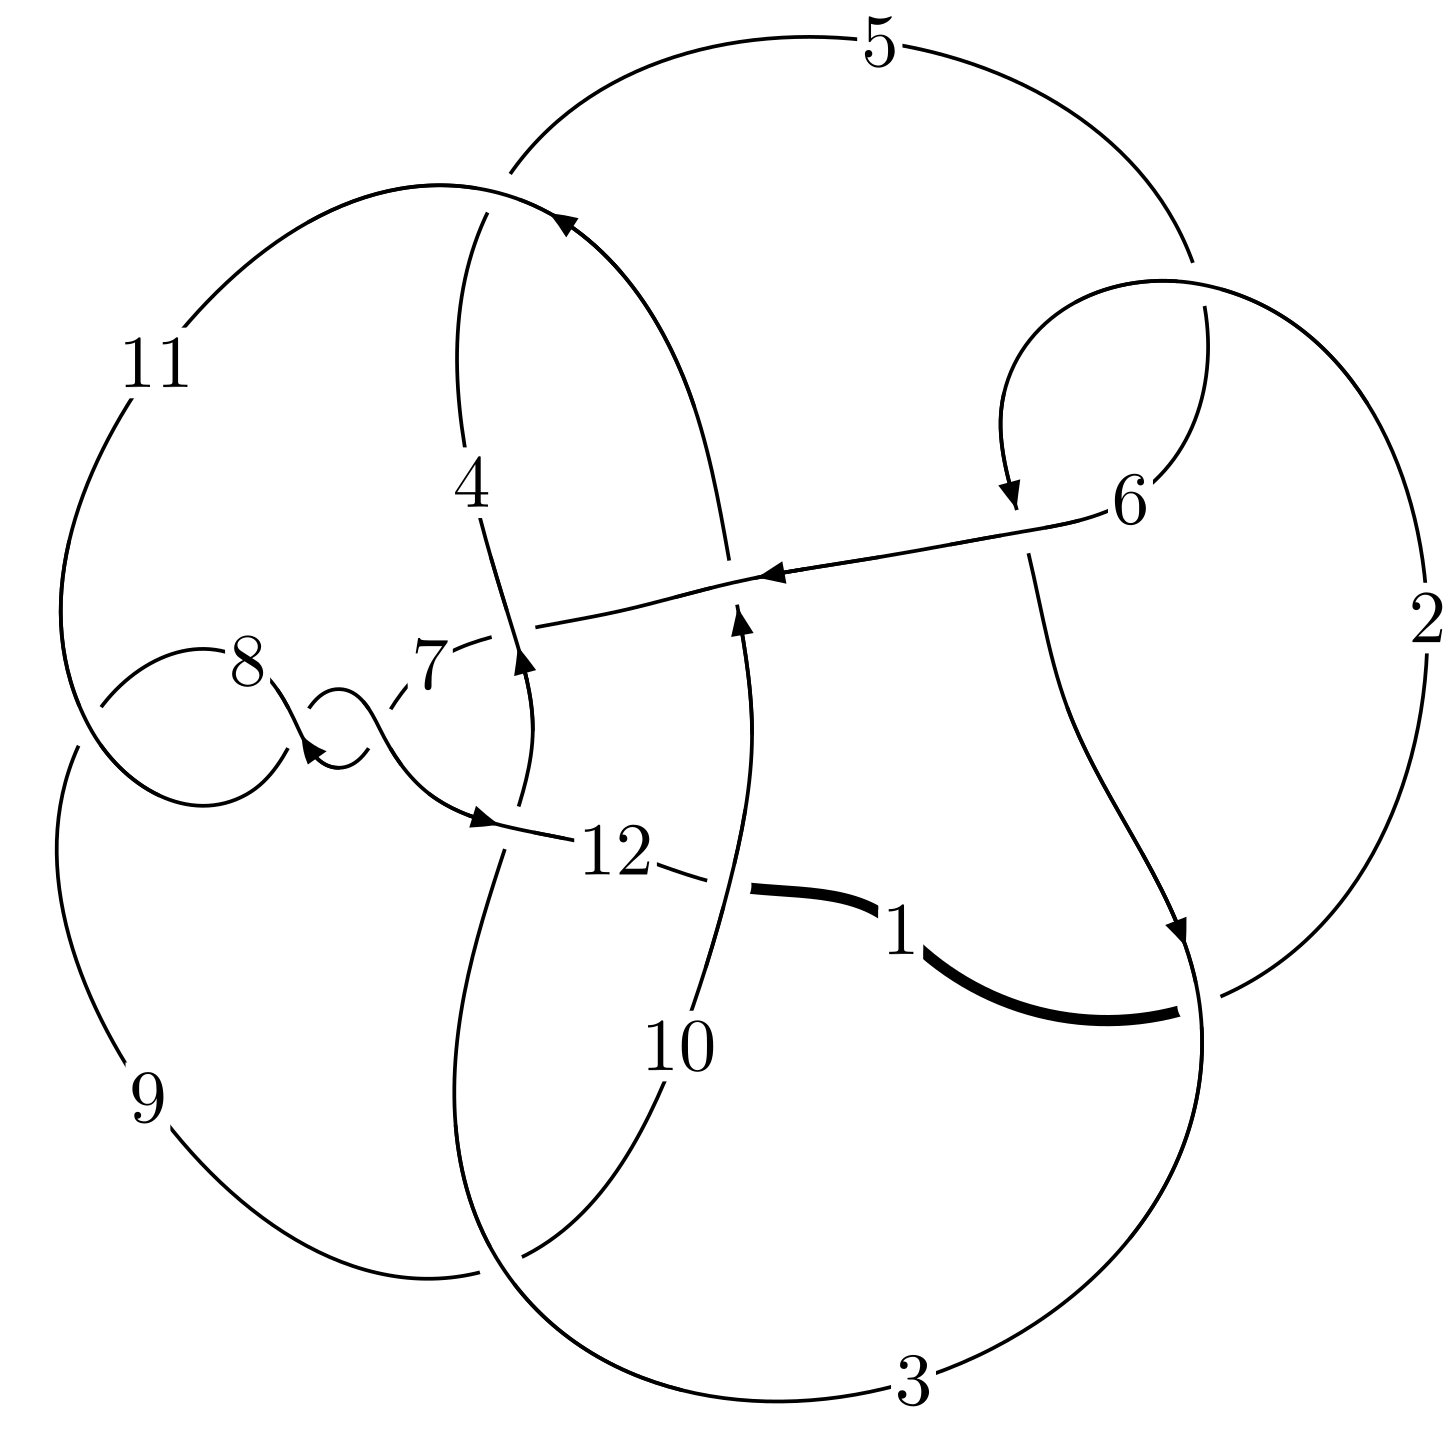
\includegraphics[width=112pt]{../../../GIT/diagram.site/Diagrams/png/2532_12n_0443.png}\\
\ \ \ A knot diagram\footnotemark}&
\allowdisplaybreaks
\textbf{Linearized knot diagam} \\
\cline{2-2}
 &
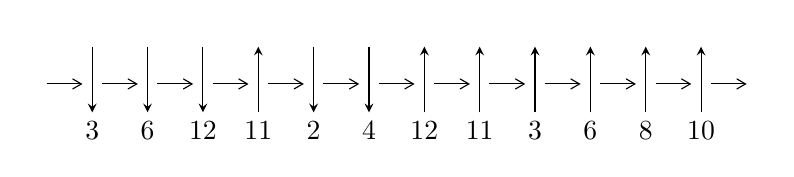
\begin{tikzpicture}[x=20pt, y=17pt]
	% nodes
	\node (C0) at (0, 0) {};
	\node (C1) at (1, 0) {};
	\node (C1U) at (1, +1) {};
	\node (C1D) at (1, -1) {3};

	\node (C2) at (2, 0) {};
	\node (C2U) at (2, +1) {};
	\node (C2D) at (2, -1) {6};

	\node (C3) at (3, 0) {};
	\node (C3U) at (3, +1) {};
	\node (C3D) at (3, -1) {12};

	\node (C4) at (4, 0) {};
	\node (C4U) at (4, +1) {};
	\node (C4D) at (4, -1) {11};

	\node (C5) at (5, 0) {};
	\node (C5U) at (5, +1) {};
	\node (C5D) at (5, -1) {2};

	\node (C6) at (6, 0) {};
	\node (C6U) at (6, +1) {};
	\node (C6D) at (6, -1) {4};

	\node (C7) at (7, 0) {};
	\node (C7U) at (7, +1) {};
	\node (C7D) at (7, -1) {12};

	\node (C8) at (8, 0) {};
	\node (C8U) at (8, +1) {};
	\node (C8D) at (8, -1) {11};

	\node (C9) at (9, 0) {};
	\node (C9U) at (9, +1) {};
	\node (C9D) at (9, -1) {3};

	\node (C10) at (10, 0) {};
	\node (C10U) at (10, +1) {};
	\node (C10D) at (10, -1) {6};

	\node (C11) at (11, 0) {};
	\node (C11U) at (11, +1) {};
	\node (C11D) at (11, -1) {8};

	\node (C12) at (12, 0) {};
	\node (C12U) at (12, +1) {};
	\node (C12D) at (12, -1) {10};
	\node (C13) at (13, 0) {};

	% arrows
	\draw[->,>={angle 60}]
	(C0) edge (C1) (C1) edge (C2) (C2) edge (C3) (C3) edge (C4) (C4) edge (C5) (C5) edge (C6) (C6) edge (C7) (C7) edge (C8) (C8) edge (C9) (C9) edge (C10) (C10) edge (C11) (C11) edge (C12) (C12) edge (C13) ;	\draw[->,>=stealth]
	(C1U) edge (C1D) (C2U) edge (C2D) (C3U) edge (C3D) (C4D) edge (C4U) (C5U) edge (C5D) (C6U) edge (C6D) (C7D) edge (C7U) (C8D) edge (C8U) (C9D) edge (C9U) (C10D) edge (C10U) (C11D) edge (C11U) (C12D) edge (C12U) ;
	\end{tikzpicture} \\
\hhline{~~} \\& 
\textbf{Solving Sequence} \\ \cline{2-2} 
 &
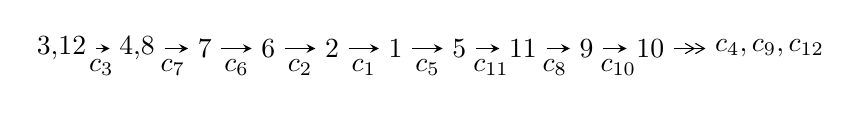
\begin{tikzpicture}[x=23pt, y=7pt]
	% node
	\node (A0) at (-1/8, 0) {3,12};
	\node (A1) at (17/16, 0) {4,8};
	\node (A2) at (17/8, 0) {7};
	\node (A3) at (25/8, 0) {6};
	\node (A4) at (33/8, 0) {2};
	\node (A5) at (41/8, 0) {1};
	\node (A6) at (49/8, 0) {5};
	\node (A7) at (57/8, 0) {11};
	\node (A8) at (65/8, 0) {9};
	\node (A9) at (73/8, 0) {10};
	\node (C1) at (1/2, -1) {$c_{3}$};
	\node (C2) at (13/8, -1) {$c_{7}$};
	\node (C3) at (21/8, -1) {$c_{6}$};
	\node (C4) at (29/8, -1) {$c_{2}$};
	\node (C5) at (37/8, -1) {$c_{1}$};
	\node (C6) at (45/8, -1) {$c_{5}$};
	\node (C7) at (53/8, -1) {$c_{11}$};
	\node (C8) at (61/8, -1) {$c_{8}$};
	\node (C9) at (69/8, -1) {$c_{10}$};
	\node (A10) at (11, 0) {$c_{4},c_{9},c_{12}$};

	% edge
	\draw[->,>=stealth]	
	(A0) edge (A1) (A1) edge (A2) (A2) edge (A3) (A3) edge (A4) (A4) edge (A5) (A5) edge (A6) (A6) edge (A7) (A7) edge (A8) (A8) edge (A9) ;
	\draw[->>,>={angle 60}]	
	(A9) edge (A10);
\end{tikzpicture} \\ 

\end{tabular} \\

\footnotetext{
The image of knot diagram is generated by the software ``\textbf{Draw programme}" developed by Andrew Bartholomew(\url{http://www.layer8.co.uk/maths/draw/index.htm\#Running-draw}), where we modified some parts for our purpose(\url{https://github.com/CATsTAILs/LinksPainter}).
}\phantom \\ \newline 
\centering \textbf{Ideals for irreducible components\footnotemark of $X_{\text{par}}$} 
 
\begin{align*}
I^u_{1}&=\langle 
b- u,\;64645 u^{14}-65427 u^{13}+\cdots+135557 a+338831,\\
\phantom{I^u_{1}}&\phantom{= \langle  }u^{15}+10 u^{13}+3 u^{12}+43 u^{11}+24 u^{10}+99 u^9+76 u^8+124 u^7+108 u^6+79 u^5+56 u^4+21 u^3+u^2-1\rangle \\
I^u_{2}&=\langle 
b+u,\;-8 u^8+3 u^7-25 u^6+25 u^5-9 u^4+26 u^3+23 u^2+a-34 u-19,\\
\phantom{I^u_{2}}&\phantom{= \langle  }u^9+3 u^7-2 u^6-3 u^4-4 u^3+3 u^2+4 u+1\rangle \\
I^u_{3}&=\langle 
80577 u^{11}-475411 u^{10}+\cdots+2674873 b-7542897,\\
\phantom{I^u_{3}}&\phantom{= \langle  }1788526 u^{11}-120225 u^{10}+\cdots+29423603 a+69597502,\\
\phantom{I^u_{3}}&\phantom{= \langle  }u^{12}-2 u^{11}+4 u^{10}-9 u^9+8 u^8-14 u^7+17 u^6-10 u^5+40 u^4- u^3+45 u^2-5 u+11\rangle \\
I^u_{4}&=\langle 
b- u-1,\;a,\;u^2+u+1\rangle \\
\\
\end{align*}
\raggedright * 4 irreducible components of $\dim_{\mathbb{C}}=0$, with total 38 representations.\\
\footnotetext{All coefficients of polynomials are rational numbers. But the coefficients are sometimes approximated in decimal forms when there is not enough margin.}
\newpage
\renewcommand{\arraystretch}{1}
\centering \section*{I. $I^u_{1}= \langle b- u,\;64645 u^{14}-65427 u^{13}+\cdots+135557 a+338831,\;u^{15}+10 u^{13}+\cdots+u^2-1 \rangle$}
\flushleft \textbf{(i) Arc colorings}\\
\begin{tabular}{m{7pt} m{180pt} m{7pt} m{180pt} }
\flushright $a_{3}=$&$\begin{pmatrix}1\\0\end{pmatrix}$ \\
\flushright $a_{12}=$&$\begin{pmatrix}0\\u\end{pmatrix}$ \\
\flushright $a_{4}=$&$\begin{pmatrix}1\\u^2\end{pmatrix}$ \\
\flushright $a_{8}=$&$\begin{pmatrix}-0.476884 u^{14}+0.482653 u^{13}+\cdots+1.81451 u-2.49955\\u\end{pmatrix}$ \\
\flushright $a_{7}=$&$\begin{pmatrix}-0.476884 u^{14}+0.482653 u^{13}+\cdots+1.81451 u-2.49955\\0.00639583 u^{14}-0.283881 u^{13}+\cdots+0.523116 u+0.482653\end{pmatrix}$ \\
\flushright $a_{6}=$&$\begin{pmatrix}-0.476884 u^{14}+0.482653 u^{13}+\cdots+2.81451 u-2.49955\\0.00639583 u^{14}-0.283881 u^{13}+\cdots+0.523116 u+0.482653\end{pmatrix}$ \\
\flushright $a_{2}=$&$\begin{pmatrix}-0.0111245 u^{14}+0.0185605 u^{13}+\cdots-0.528095 u+2.36120\\0.205168 u^{14}-0.302522 u^{13}+\cdots-0.493778 u+0.0121646\end{pmatrix}$ \\
\flushright $a_{1}=$&$\begin{pmatrix}0.194044 u^{14}-0.283962 u^{13}+\cdots-1.02187 u+2.37336\\0.205168 u^{14}-0.302522 u^{13}+\cdots-0.493778 u+0.0121646\end{pmatrix}$ \\
\flushright $a_{5}=$&$\begin{pmatrix}-0.879586 u^{14}-0.206208 u^{13}+\cdots+4.63070 u-0.816210\\-0.198691 u^{14}+0.0715566 u^{13}+\cdots+0.126183 u+0.282840\end{pmatrix}$ \\
\flushright $a_{11}=$&$\begin{pmatrix}0.897106 u^{14}-0.0962326 u^{13}+\cdots-5.57949 u-2.06234\\-0.00639583 u^{14}+0.283881 u^{13}+\cdots+1.47688 u-0.482653\end{pmatrix}$ \\
\flushright $a_{9}=$&$\begin{pmatrix}0.475313 u^{14}-0.416371 u^{13}+\cdots-7.11258 u+0.678549\\0.0187228 u^{14}+0.0271177 u^{13}+\cdots+0.579778 u-0.386420\end{pmatrix}$ \\
\flushright $a_{10}=$&$\begin{pmatrix}0.494036 u^{14}-0.389253 u^{13}+\cdots-6.53280 u+0.292128\\0.0187228 u^{14}+0.0271177 u^{13}+\cdots+0.579778 u-0.386420\end{pmatrix}$\\&\end{tabular}
\flushleft \textbf{(ii) Obstruction class $= -1$}\\~\\
\flushleft \textbf{(iii) Cusp Shapes $= \frac{335739}{135557} u^{14}-\frac{152409}{135557} u^{13}+\cdots+\frac{281645}{135557} u+\frac{754781}{135557}$}\\~\\
\newpage\renewcommand{\arraystretch}{1}
\flushleft \textbf{(iv) u-Polynomials at the component}\newline \\
\begin{tabular}{m{50pt}|m{274pt}}
Crossings & \hspace{64pt}u-Polynomials at each crossing \\
\hline $$\begin{aligned}c_{1}\end{aligned}$$&$\begin{aligned}
&u^{15}+20 u^{14}+\cdots+849 u+16
\end{aligned}$\\
\hline $$\begin{aligned}c_{2},c_{5}\end{aligned}$$&$\begin{aligned}
&u^{15}+8 u^{14}+\cdots+23 u-4
\end{aligned}$\\
\hline $$\begin{aligned}c_{3},c_{6}\end{aligned}$$&$\begin{aligned}
&u^{15}+10 u^{13}+\cdots+u^2-1
\end{aligned}$\\
\hline $$\begin{aligned}c_{4},c_{9}\end{aligned}$$&$\begin{aligned}
&u^{15}+13 u^{13}+\cdots+u-1
\end{aligned}$\\
\hline $$\begin{aligned}c_{7},c_{8},c_{11}\end{aligned}$$&$\begin{aligned}
&u^{15}+6 u^{14}+\cdots-5 u-2
\end{aligned}$\\
\hline $$\begin{aligned}c_{10},c_{12}\end{aligned}$$&$\begin{aligned}
&u^{15}- u^{14}+\cdots-11 u-1
\end{aligned}$\\
\hline
\end{tabular}\\~\\
\newpage\renewcommand{\arraystretch}{1}
\flushleft \textbf{(v) Riley Polynomials at the component}\newline \\
\begin{tabular}{m{50pt}|m{274pt}}
Crossings & \hspace{64pt}Riley Polynomials at each crossing \\
\hline $$\begin{aligned}c_{1}\end{aligned}$$&$\begin{aligned}
&y^{15}-44 y^{14}+\cdots+606753 y-256
\end{aligned}$\\
\hline $$\begin{aligned}c_{2},c_{5}\end{aligned}$$&$\begin{aligned}
&y^{15}-20 y^{14}+\cdots+849 y-16
\end{aligned}$\\
\hline $$\begin{aligned}c_{3},c_{6}\end{aligned}$$&$\begin{aligned}
&y^{15}+20 y^{14}+\cdots+2 y-1
\end{aligned}$\\
\hline $$\begin{aligned}c_{4},c_{9}\end{aligned}$$&$\begin{aligned}
&y^{15}+26 y^{14}+\cdots-3 y-1
\end{aligned}$\\
\hline $$\begin{aligned}c_{7},c_{8},c_{11}\end{aligned}$$&$\begin{aligned}
&y^{15}+10 y^{14}+\cdots-39 y-4
\end{aligned}$\\
\hline $$\begin{aligned}c_{10},c_{12}\end{aligned}$$&$\begin{aligned}
&y^{15}+19 y^{14}+\cdots+95 y-1
\end{aligned}$\\
\hline
\end{tabular}\\~\\
\newpage\flushleft \textbf{(vi) Complex Volumes and Cusp Shapes}
$$\begin{array}{c|c|c}  
\text{Solutions to }I^u_{1}& \I (\text{vol} + \sqrt{-1}CS) & \text{Cusp shape}\\
 \hline 
\begin{aligned}
u &= \phantom{-}0.045427 + 1.039060 I \\
a &= \phantom{-}1.54244 - 0.28684 I \\
b &= \phantom{-}0.045427 + 1.039060 I\end{aligned}
 & -11.28150 + 1.93400 I & -1.23160 - 1.02985 I \\ \hline\begin{aligned}
u &= \phantom{-}0.045427 - 1.039060 I \\
a &= \phantom{-}1.54244 + 0.28684 I \\
b &= \phantom{-}0.045427 - 1.039060 I\end{aligned}
 & -11.28150 - 1.93400 I & -1.23160 + 1.02985 I \\ \hline\begin{aligned}
u &= -0.608111 + 0.211954 I \\
a &= \phantom{-}0.250704 - 0.629982 I \\
b &= -0.608111 + 0.211954 I\end{aligned}
 & -1.45492 + 0.35788 I & -5.52968 - 1.62247 I \\ \hline\begin{aligned}
u &= -0.608111 - 0.211954 I \\
a &= \phantom{-}0.250704 + 0.629982 I \\
b &= -0.608111 - 0.211954 I\end{aligned}
 & -1.45492 - 0.35788 I & -5.52968 + 1.62247 I \\ \hline\begin{aligned}
u &= \phantom{-}0.06518 + 1.45860 I \\
a &= -0.406098 - 0.405536 I \\
b &= \phantom{-}0.06518 + 1.45860 I\end{aligned}
 & \phantom{-}3.63562 + 1.34338 I & \phantom{-}2.60619 - 3.21341 I \\ \hline\begin{aligned}
u &= \phantom{-}0.06518 - 1.45860 I \\
a &= -0.406098 + 0.405536 I \\
b &= \phantom{-}0.06518 - 1.45860 I\end{aligned}
 & \phantom{-}3.63562 - 1.34338 I & \phantom{-}2.60619 + 3.21341 I \\ \hline\begin{aligned}
u &= -0.094803 + 0.399698 I \\
a &= -3.16771 + 0.99078 I \\
b &= -0.094803 + 0.399698 I\end{aligned}
 & -3.74744 + 2.10465 I & \phantom{-}5.87690 - 3.70353 I \\ \hline\begin{aligned}
u &= -0.094803 - 0.399698 I \\
a &= -3.16771 - 0.99078 I \\
b &= -0.094803 - 0.399698 I\end{aligned}
 & -3.74744 - 2.10465 I & \phantom{-}5.87690 + 3.70353 I \\ \hline\begin{aligned}
u &= \phantom{-}0.23646 + 1.59594 I \\
a &= \phantom{-}0.306052 - 0.769874 I \\
b &= \phantom{-}0.23646 + 1.59594 I\end{aligned}
 & -4.76135 - 4.08820 I & \phantom{-}0.76517 + 2.11409 I \\ \hline\begin{aligned}
u &= \phantom{-}0.23646 - 1.59594 I \\
a &= \phantom{-}0.306052 + 0.769874 I \\
b &= \phantom{-}0.23646 - 1.59594 I\end{aligned}
 & -4.76135 + 4.08820 I & \phantom{-}0.76517 - 2.11409 I\\
 \hline 
 \end{array}$$\newpage$$\begin{array}{c|c|c}  
\text{Solutions to }I^u_{1}& \I (\text{vol} + \sqrt{-1}CS) & \text{Cusp shape}\\
 \hline 
\begin{aligned}
u &= -0.47405 + 1.56562 I \\
a &= \phantom{-}0.532315 - 0.431362 I \\
b &= -0.47405 + 1.56562 I\end{aligned}
 & \phantom{-}2.30289 + 5.28134 I & -1.29339 - 3.24953 I \\ \hline\begin{aligned}
u &= -0.47405 - 1.56562 I \\
a &= \phantom{-}0.532315 + 0.431362 I \\
b &= -0.47405 - 1.56562 I\end{aligned}
 & \phantom{-}2.30289 - 5.28134 I & -1.29339 + 3.24953 I \\ \hline\begin{aligned}
u &= \phantom{-}0.273398\phantom{ +0.000000I} \\
a &= -2.01535\phantom{ +0.000000I} \\
b &= \phantom{-}0.273398\phantom{ +0.000000I}\end{aligned}
 & \phantom{-}0.899032\phantom{ +0.000000I} & \phantom{-}11.1030\phantom{ +0.000000I} \\ \hline\begin{aligned}
u &= \phantom{-}0.69320 + 1.66542 I \\
a &= -0.550040 - 0.669032 I \\
b &= \phantom{-}0.69320 + 1.66542 I\end{aligned}
 & -8.17186 - 11.29110 I & -0.74494 + 5.10967 I \\ \hline\begin{aligned}
u &= \phantom{-}0.69320 - 1.66542 I \\
a &= -0.550040 + 0.669032 I \\
b &= \phantom{-}0.69320 - 1.66542 I\end{aligned}
 & -8.17186 + 11.29110 I & -0.74494 - 5.10967 I\\
 \hline 
 \end{array}$$\newpage\newpage\renewcommand{\arraystretch}{1}
\centering \section*{II. $I^u_{2}= \langle b+u,\;-8 u^8+3 u^7+\cdots+a-19,\;u^9+3 u^7-2 u^6-3 u^4-4 u^3+3 u^2+4 u+1 \rangle$}
\flushleft \textbf{(i) Arc colorings}\\
\begin{tabular}{m{7pt} m{180pt} m{7pt} m{180pt} }
\flushright $a_{3}=$&$\begin{pmatrix}1\\0\end{pmatrix}$ \\
\flushright $a_{12}=$&$\begin{pmatrix}0\\u\end{pmatrix}$ \\
\flushright $a_{4}=$&$\begin{pmatrix}1\\u^2\end{pmatrix}$ \\
\flushright $a_{8}=$&$\begin{pmatrix}8 u^8-3 u^7+25 u^6-25 u^5+9 u^4-26 u^3-23 u^2+34 u+19\\- u\end{pmatrix}$ \\
\flushright $a_{7}=$&$\begin{pmatrix}8 u^8-3 u^7+25 u^6-25 u^5+9 u^4-26 u^3-23 u^2+34 u+19\\u^8+3 u^6-2 u^5-2 u^3-4 u^2+3 u+3\end{pmatrix}$ \\
\flushright $a_{6}=$&$\begin{pmatrix}8 u^8-3 u^7+25 u^6-25 u^5+9 u^4-26 u^3-23 u^2+33 u+19\\u^8+3 u^6-2 u^5-3 u^3-4 u^2+3 u+3\end{pmatrix}$ \\
\flushright $a_{2}=$&$\begin{pmatrix}-11 u^8+5 u^7-35 u^6+38 u^5-16 u^4+40 u^3+27 u^2-47 u-23\\-2 u^8+u^7-6 u^6+7 u^5-2 u^4+6 u^3+5 u^2-10 u-6\end{pmatrix}$ \\
\flushright $a_{1}=$&$\begin{pmatrix}-13 u^8+6 u^7-41 u^6+45 u^5-18 u^4+46 u^3+32 u^2-57 u-29\\-2 u^8+u^7-6 u^6+7 u^5-2 u^4+6 u^3+5 u^2-10 u-6\end{pmatrix}$ \\
\flushright $a_{5}=$&$\begin{pmatrix}-4 u^8+3 u^7-14 u^6+18 u^5-13 u^4+19 u^3+2 u^2-16 u-3\\-3 u^8+u^7-10 u^6+9 u^5-5 u^4+11 u^3+9 u^2-10 u-5\end{pmatrix}$ \\
\flushright $a_{11}=$&$\begin{pmatrix}14 u^8-8 u^7+46 u^6-54 u^5+29 u^4-57 u^3-25 u^2+58 u+24\\u^8+3 u^6-2 u^5-2 u^3-4 u^2+5 u+3\end{pmatrix}$ \\
\flushright $a_{9}=$&$\begin{pmatrix}4 u^8-3 u^7+14 u^6-18 u^5+13 u^4-20 u^3-2 u^2+14 u+4\\3 u^8-2 u^7+10 u^6-13 u^5+7 u^4-14 u^3-4 u^2+13 u+5\end{pmatrix}$ \\
\flushright $a_{10}=$&$\begin{pmatrix}7 u^8-5 u^7+24 u^6-31 u^5+20 u^4-34 u^3-6 u^2+27 u+9\\3 u^8-2 u^7+10 u^6-13 u^5+7 u^4-14 u^3-4 u^2+13 u+5\end{pmatrix}$\\&\end{tabular}
\flushleft \textbf{(ii) Obstruction class $= 1$}\\~\\
\flushleft \textbf{(iii) Cusp Shapes $= 37 u^8-21 u^7+123 u^6-143 u^5+80 u^4-154 u^3-65 u^2+148 u+61$}\\~\\
\newpage\renewcommand{\arraystretch}{1}
\flushleft \textbf{(iv) u-Polynomials at the component}\newline \\
\begin{tabular}{m{50pt}|m{274pt}}
Crossings & \hspace{64pt}u-Polynomials at each crossing \\
\hline $$\begin{aligned}c_{1}\end{aligned}$$&$\begin{aligned}
&u^9-11 u^8+\cdots+105 u-25
\end{aligned}$\\
\hline $$\begin{aligned}c_{2}\end{aligned}$$&$\begin{aligned}
&u^9+5 u^8+7 u^7-3 u^6-14 u^5-4 u^4+13 u^3+8 u^2-5 u-5
\end{aligned}$\\
\hline $$\begin{aligned}c_{3},c_{6}\end{aligned}$$&$\begin{aligned}
&u^9+3 u^7-2 u^6-3 u^4-4 u^3+3 u^2+4 u+1
\end{aligned}$\\
\hline $$\begin{aligned}c_{4},c_{9}\end{aligned}$$&$\begin{aligned}
&u^9+4 u^7-4 u^5+7 u^4+3 u^3-4 u^2+u+1
\end{aligned}$\\
\hline $$\begin{aligned}c_{5}\end{aligned}$$&$\begin{aligned}
&u^9-5 u^8+7 u^7+3 u^6-14 u^5+4 u^4+13 u^3-8 u^2-5 u+5
\end{aligned}$\\
\hline $$\begin{aligned}c_{7},c_{8}\end{aligned}$$&$\begin{aligned}
&u^9+3 u^8+8 u^7+13 u^6+20 u^5+22 u^4+23 u^3+17 u^2+11 u+3
\end{aligned}$\\
\hline $$\begin{aligned}c_{10},c_{12}\end{aligned}$$&$\begin{aligned}
&u^9+u^8+5 u^7+6 u^6+8 u^5- u^3-3 u^2- u-1
\end{aligned}$\\
\hline $$\begin{aligned}c_{11}\end{aligned}$$&$\begin{aligned}
&u^9-3 u^8+8 u^7-13 u^6+20 u^5-22 u^4+23 u^3-17 u^2+11 u-3
\end{aligned}$\\
\hline
\end{tabular}\\~\\
\newpage\renewcommand{\arraystretch}{1}
\flushleft \textbf{(v) Riley Polynomials at the component}\newline \\
\begin{tabular}{m{50pt}|m{274pt}}
Crossings & \hspace{64pt}Riley Polynomials at each crossing \\
\hline $$\begin{aligned}c_{1}\end{aligned}$$&$\begin{aligned}
&y^9-19 y^8+\cdots-675 y-625
\end{aligned}$\\
\hline $$\begin{aligned}c_{2},c_{5}\end{aligned}$$&$\begin{aligned}
&y^9-11 y^8+\cdots+105 y-25
\end{aligned}$\\
\hline $$\begin{aligned}c_{3},c_{6}\end{aligned}$$&$\begin{aligned}
&y^9+6 y^8+9 y^7-12 y^6-28 y^5+27 y^4+38 y^3-35 y^2+10 y-1
\end{aligned}$\\
\hline $$\begin{aligned}c_{4},c_{9}\end{aligned}$$&$\begin{aligned}
&y^9+8 y^8+8 y^7-26 y^6+42 y^5-65 y^4+57 y^3-24 y^2+9 y-1
\end{aligned}$\\
\hline $$\begin{aligned}c_{7},c_{8},c_{11}\end{aligned}$$&$\begin{aligned}
&y^9+7 y^8+26 y^7+65 y^6+116 y^5+152 y^4+143 y^3+85 y^2+19 y-9
\end{aligned}$\\
\hline $$\begin{aligned}c_{10},c_{12}\end{aligned}$$&$\begin{aligned}
&y^9+9 y^8+29 y^7+42 y^6+58 y^5+12 y^4-3 y^3-7 y^2-5 y-1
\end{aligned}$\\
\hline
\end{tabular}\\~\\
\newpage\flushleft \textbf{(vi) Complex Volumes and Cusp Shapes}
$$\begin{array}{c|c|c}  
\text{Solutions to }I^u_{2}& \I (\text{vol} + \sqrt{-1}CS) & \text{Cusp shape}\\
 \hline 
\begin{aligned}
u &= \phantom{-}1.060910 + 0.248265 I \\
a &= \phantom{-}0.603246 + 0.904793 I \\
b &= -1.060910 - 0.248265 I\end{aligned}
 & -14.5038 + 1.7038 I & -5.12137 - 0.30387 I \\ \hline\begin{aligned}
u &= \phantom{-}1.060910 - 0.248265 I \\
a &= \phantom{-}0.603246 - 0.904793 I \\
b &= -1.060910 + 0.248265 I\end{aligned}
 & -14.5038 - 1.7038 I & -5.12137 + 0.30387 I \\ \hline\begin{aligned}
u &= -0.513365 + 0.121815 I \\
a &= -0.35477 + 2.45080 I \\
b &= \phantom{-}0.513365 - 0.121815 I\end{aligned}
 & -4.37176 + 2.01399 I & -7.44425 - 1.80958 I \\ \hline\begin{aligned}
u &= -0.513365 - 0.121815 I \\
a &= -0.35477 - 2.45080 I \\
b &= \phantom{-}0.513365 + 0.121815 I\end{aligned}
 & -4.37176 - 2.01399 I & -7.44425 + 1.80958 I \\ \hline\begin{aligned}
u &= \phantom{-}0.12963 + 1.46755 I \\
a &= \phantom{-}0.724641 + 0.570324 I \\
b &= -0.12963 - 1.46755 I\end{aligned}
 & \phantom{-}3.37793 - 0.60932 I & \phantom{-}0.678183 + 0.313757 I \\ \hline\begin{aligned}
u &= \phantom{-}0.12963 - 1.46755 I \\
a &= \phantom{-}0.724641 - 0.570324 I \\
b &= -0.12963 + 1.46755 I\end{aligned}
 & \phantom{-}3.37793 + 0.60932 I & \phantom{-}0.678183 - 0.313757 I \\ \hline\begin{aligned}
u &= -0.524571\phantom{ +0.000000I} \\
a &= \phantom{-}0.862725\phantom{ +0.000000I} \\
b &= \phantom{-}0.524571\phantom{ +0.000000I}\end{aligned}
 & -0.323696\phantom{ +0.000000I} & \phantom{-}2.44920\phantom{ +0.000000I} \\ \hline\begin{aligned}
u &= -0.41489 + 1.57652 I \\
a &= -0.404481 + 0.632682 I \\
b &= \phantom{-}0.41489 - 1.57652 I\end{aligned}
 & \phantom{-}4.14493 + 5.44292 I & \phantom{-}3.66282 - 5.29674 I \\ \hline\begin{aligned}
u &= -0.41489 - 1.57652 I \\
a &= -0.404481 - 0.632682 I \\
b &= \phantom{-}0.41489 + 1.57652 I\end{aligned}
 & \phantom{-}4.14493 - 5.44292 I & \phantom{-}3.66282 + 5.29674 I\\
 \hline 
 \end{array}$$\newpage\newpage\renewcommand{\arraystretch}{1}
\centering \section*{III. $I^u_{3}= \langle 8.06\times10^{4} u^{11}-4.75\times10^{5} u^{10}+\cdots+2.67\times10^{6} b-7.54\times10^{6},\;1.79\times10^{6} u^{11}-1.20\times10^{5} u^{10}+\cdots+2.94\times10^{7} a+6.96\times10^{7},\;u^{12}-2 u^{11}+\cdots-5 u+11 \rangle$}
\flushleft \textbf{(i) Arc colorings}\\
\begin{tabular}{m{7pt} m{180pt} m{7pt} m{180pt} }
\flushright $a_{3}=$&$\begin{pmatrix}1\\0\end{pmatrix}$ \\
\flushright $a_{12}=$&$\begin{pmatrix}0\\u\end{pmatrix}$ \\
\flushright $a_{4}=$&$\begin{pmatrix}1\\u^2\end{pmatrix}$ \\
\flushright $a_{8}=$&$\begin{pmatrix}-0.0607854 u^{11}+0.00408601 u^{10}+\cdots-2.36373 u-2.36536\\-0.0301237 u^{11}+0.177732 u^{10}+\cdots-1.72718 u+2.81991\end{pmatrix}$ \\
\flushright $a_{7}=$&$\begin{pmatrix}-0.0607854 u^{11}+0.00408601 u^{10}+\cdots-2.36373 u-2.36536\\-0.0213565 u^{11}+0.254975 u^{10}+\cdots-1.64596 u+4.11224\end{pmatrix}$ \\
\flushright $a_{6}=$&$\begin{pmatrix}-0.0909091 u^{11}+0.181818 u^{10}+\cdots-4.09091 u+0.454545\\-0.0301237 u^{11}+0.177732 u^{10}+\cdots-0.727180 u+2.81991\end{pmatrix}$ \\
\flushright $a_{2}=$&$\begin{pmatrix}0.256355 u^{11}-0.482587 u^{10}+\cdots+7.74069 u+0.445403\\-0.00489332 u^{11}-0.0509161 u^{10}+\cdots-0.643385 u-4.28738\end{pmatrix}$ \\
\flushright $a_{1}=$&$\begin{pmatrix}0.251462 u^{11}-0.533503 u^{10}+\cdots+7.09731 u-3.84198\\-0.00489332 u^{11}-0.0509161 u^{10}+\cdots-0.643385 u-4.28738\end{pmatrix}$ \\
\flushright $a_{5}=$&$\begin{pmatrix}0.268729 u^{11}-0.424867 u^{10}+\cdots+9.92533 u+0.682260\\0.0431217 u^{11}-0.254037 u^{10}+\cdots-1.36716 u-6.19453\end{pmatrix}$ \\
\flushright $a_{11}=$&$\begin{pmatrix}-0.0475752 u^{11}+0.137019 u^{10}+\cdots-1.83773 u+2.65443\\0.108361 u^{11}-0.141105 u^{10}+\cdots+5.20146 u-0.289069\end{pmatrix}$ \\
\flushright $a_{9}=$&$\begin{pmatrix}0.107514 u^{11}-0.277645 u^{10}+\cdots+3.09999 u-2.88464\\-0.159615 u^{11}+0.245201 u^{10}+\cdots-5.43439 u-0.607579\end{pmatrix}$ \\
\flushright $a_{10}=$&$\begin{pmatrix}-0.0521010 u^{11}-0.0324441 u^{10}+\cdots-2.33440 u-3.49222\\-0.159615 u^{11}+0.245201 u^{10}+\cdots-5.43439 u-0.607579\end{pmatrix}$\\&\end{tabular}
\flushleft \textbf{(ii) Obstruction class $= -1$}\\~\\
\flushleft \textbf{(iii) Cusp Shapes $= \frac{364002}{2674873} u^{11}-\frac{239807}{2674873} u^{10}+\cdots+\frac{14456768}{2674873} u+\frac{4628741}{2674873}$}\\~\\
\newpage\renewcommand{\arraystretch}{1}
\flushleft \textbf{(iv) u-Polynomials at the component}\newline \\
\begin{tabular}{m{50pt}|m{274pt}}
Crossings & \hspace{64pt}u-Polynomials at each crossing \\
\hline $$\begin{aligned}c_{1}\end{aligned}$$&$\begin{aligned}
&(u^6+10 u^5+37 u^4+63 u^3+50 u^2+8 u+1)^2
\end{aligned}$\\
\hline $$\begin{aligned}c_{2},c_{5}\end{aligned}$$&$\begin{aligned}
&(u^6-2 u^5-3 u^4+5 u^3+4 u^2-4 u+1)^2
\end{aligned}$\\
\hline $$\begin{aligned}c_{3},c_{6}\end{aligned}$$&$\begin{aligned}
&u^{12}-2 u^{11}+\cdots-5 u+11
\end{aligned}$\\
\hline $$\begin{aligned}c_{4},c_{9}\end{aligned}$$&$\begin{aligned}
&u^{12}+10 u^{10}+\cdots+21 u+85
\end{aligned}$\\
\hline $$\begin{aligned}c_{7},c_{8},c_{11}\end{aligned}$$&$\begin{aligned}
&(u^6- u^5+2 u^4- u^3+3 u^2- u+2)^2
\end{aligned}$\\
\hline $$\begin{aligned}c_{10},c_{12}\end{aligned}$$&$\begin{aligned}
&u^{12}+3 u^{11}+\cdots+34 u+97
\end{aligned}$\\
\hline
\end{tabular}\\~\\
\newpage\renewcommand{\arraystretch}{1}
\flushleft \textbf{(v) Riley Polynomials at the component}\newline \\
\begin{tabular}{m{50pt}|m{274pt}}
Crossings & \hspace{64pt}Riley Polynomials at each crossing \\
\hline $$\begin{aligned}c_{1}\end{aligned}$$&$\begin{aligned}
&(y^6-26 y^5+209 y^4-427 y^3+1566 y^2+36 y+1)^2
\end{aligned}$\\
\hline $$\begin{aligned}c_{2},c_{5}\end{aligned}$$&$\begin{aligned}
&(y^6-10 y^5+37 y^4-63 y^3+50 y^2-8 y+1)^2
\end{aligned}$\\
\hline $$\begin{aligned}c_{3},c_{6}\end{aligned}$$&$\begin{aligned}
&y^{12}+4 y^{11}+\cdots+965 y+121
\end{aligned}$\\
\hline $$\begin{aligned}c_{4},c_{9}\end{aligned}$$&$\begin{aligned}
&y^{12}+20 y^{11}+\cdots+4489 y+7225
\end{aligned}$\\
\hline $$\begin{aligned}c_{7},c_{8},c_{11}\end{aligned}$$&$\begin{aligned}
&(y^6+3 y^5+8 y^4+13 y^3+15 y^2+11 y+4)^2
\end{aligned}$\\
\hline $$\begin{aligned}c_{10},c_{12}\end{aligned}$$&$\begin{aligned}
&y^{12}+13 y^{11}+\cdots+6410 y+9409
\end{aligned}$\\
\hline
\end{tabular}\\~\\
\newpage\flushleft \textbf{(vi) Complex Volumes and Cusp Shapes}
$$\begin{array}{c|c|c}  
\text{Solutions to }I^u_{3}& \I (\text{vol} + \sqrt{-1}CS) & \text{Cusp shape}\\
 \hline 
\begin{aligned}
u &= -0.954376 + 0.767237 I \\
a &= -0.347916 + 0.700187 I \\
b &= -0.288553 - 1.211850 I\end{aligned}
 & -1.32320 + 0.88172 I & -1.96296 - 1.82677 I \\ \hline\begin{aligned}
u &= -0.954376 - 0.767237 I \\
a &= -0.347916 - 0.700187 I \\
b &= -0.288553 + 1.211850 I\end{aligned}
 & -1.32320 - 0.88172 I & -1.96296 + 1.82677 I \\ \hline\begin{aligned}
u &= -0.288553 + 1.211850 I \\
a &= \phantom{-}0.768435 - 0.013672 I \\
b &= -0.954376 - 0.767237 I\end{aligned}
 & -1.32320 - 0.88172 I & -1.96296 + 1.82677 I \\ \hline\begin{aligned}
u &= -0.288553 - 1.211850 I \\
a &= \phantom{-}0.768435 + 0.013672 I \\
b &= -0.954376 + 0.767237 I\end{aligned}
 & -1.32320 + 0.88172 I & -1.96296 - 1.82677 I \\ \hline\begin{aligned}
u &= \phantom{-}0.507879 + 1.312290 I \\
a &= \phantom{-}0.416941 + 0.844475 I \\
b &= -0.16044 - 1.50723 I\end{aligned}
 & \phantom{-}3.57385 - 3.35669 I & \phantom{-}1.80671 + 2.26936 I \\ \hline\begin{aligned}
u &= \phantom{-}0.507879 - 1.312290 I \\
a &= \phantom{-}0.416941 - 0.844475 I \\
b &= -0.16044 + 1.50723 I\end{aligned}
 & \phantom{-}3.57385 + 3.35669 I & \phantom{-}1.80671 - 2.26936 I \\ \hline\begin{aligned}
u &= \phantom{-}0.102054 + 0.545648 I \\
a &= -1.46225 - 1.37604 I \\
b &= \phantom{-}1.79344 - 0.39470 I\end{aligned}
 & -12.94270 - 2.40920 I & \phantom{-}0.65626 + 2.92591 I \\ \hline\begin{aligned}
u &= \phantom{-}0.102054 - 0.545648 I \\
a &= -1.46225 + 1.37604 I \\
b &= \phantom{-}1.79344 + 0.39470 I\end{aligned}
 & -12.94270 + 2.40920 I & \phantom{-}0.65626 - 2.92591 I \\ \hline\begin{aligned}
u &= -0.16044 + 1.50723 I \\
a &= -0.577713 + 0.656253 I \\
b &= \phantom{-}0.507879 - 1.312290 I\end{aligned}
 & \phantom{-}3.57385 + 3.35669 I & \phantom{-}1.80671 - 2.26936 I \\ \hline\begin{aligned}
u &= -0.16044 - 1.50723 I \\
a &= -0.577713 - 0.656253 I \\
b &= \phantom{-}0.507879 + 1.312290 I\end{aligned}
 & \phantom{-}3.57385 - 3.35669 I & \phantom{-}1.80671 + 2.26936 I\\
 \hline 
 \end{array}$$\newpage$$\begin{array}{c|c|c}  
\text{Solutions to }I^u_{3}& \I (\text{vol} + \sqrt{-1}CS) & \text{Cusp shape}\\
 \hline 
\begin{aligned}
u &= \phantom{-}1.79344 + 0.39470 I \\
a &= \phantom{-}0.429775 + 0.428603 I \\
b &= \phantom{-}0.102054 - 0.545648 I\end{aligned}
 & -12.94270 + 2.40920 I & \phantom{-}0.65626 - 2.92591 I \\ \hline\begin{aligned}
u &= \phantom{-}1.79344 - 0.39470 I \\
a &= \phantom{-}0.429775 - 0.428603 I \\
b &= \phantom{-}0.102054 + 0.545648 I\end{aligned}
 & -12.94270 - 2.40920 I & \phantom{-}0.65626 + 2.92591 I\\
 \hline 
 \end{array}$$\newpage\newpage\renewcommand{\arraystretch}{1}
\centering \section*{IV. $I^u_{4}= \langle b- u-1,\;a,\;u^2+u+1 \rangle$}
\flushleft \textbf{(i) Arc colorings}\\
\begin{tabular}{m{7pt} m{180pt} m{7pt} m{180pt} }
\flushright $a_{3}=$&$\begin{pmatrix}1\\0\end{pmatrix}$ \\
\flushright $a_{12}=$&$\begin{pmatrix}0\\u\end{pmatrix}$ \\
\flushright $a_{4}=$&$\begin{pmatrix}1\\- u-1\end{pmatrix}$ \\
\flushright $a_{8}=$&$\begin{pmatrix}0\\u+1\end{pmatrix}$ \\
\flushright $a_{7}=$&$\begin{pmatrix}0\\u+1\end{pmatrix}$ \\
\flushright $a_{6}=$&$\begin{pmatrix}u+1\\1\end{pmatrix}$ \\
\flushright $a_{2}=$&$\begin{pmatrix}- u\\-1\end{pmatrix}$ \\
\flushright $a_{1}=$&$\begin{pmatrix}- u-1\\-1\end{pmatrix}$ \\
\flushright $a_{5}=$&$\begin{pmatrix}1\\0\end{pmatrix}$ \\
\flushright $a_{11}=$&$\begin{pmatrix}0\\u\end{pmatrix}$ \\
\flushright $a_{9}=$&$\begin{pmatrix}0\\u+1\end{pmatrix}$ \\
\flushright $a_{10}=$&$\begin{pmatrix}u+1\\u+1\end{pmatrix}$\\&\end{tabular}
\flushleft \textbf{(ii) Obstruction class $= 1$}\\~\\
\flushleft \textbf{(iii) Cusp Shapes $= 3$}\\~\\
\newpage\renewcommand{\arraystretch}{1}
\flushleft \textbf{(iv) u-Polynomials at the component}\newline \\
\begin{tabular}{m{50pt}|m{274pt}}
Crossings & \hspace{64pt}u-Polynomials at each crossing \\
\hline $$\begin{aligned}c_{1},c_{2},c_{10}\\c_{12}\end{aligned}$$&$\begin{aligned}
&(u-1)^2
\end{aligned}$\\
\hline $$\begin{aligned}c_{3},c_{4},c_{6}\\c_{9}\end{aligned}$$&$\begin{aligned}
&u^2+u+1
\end{aligned}$\\
\hline $$\begin{aligned}c_{5}\end{aligned}$$&$\begin{aligned}
&(u+1)^2
\end{aligned}$\\
\hline $$\begin{aligned}c_{7},c_{8},c_{11}\end{aligned}$$&$\begin{aligned}
&u^2
\end{aligned}$\\
\hline
\end{tabular}\\~\\
\newpage\renewcommand{\arraystretch}{1}
\flushleft \textbf{(v) Riley Polynomials at the component}\newline \\
\begin{tabular}{m{50pt}|m{274pt}}
Crossings & \hspace{64pt}Riley Polynomials at each crossing \\
\hline $$\begin{aligned}c_{1},c_{2},c_{5}\\c_{10},c_{12}\end{aligned}$$&$\begin{aligned}
&(y-1)^2
\end{aligned}$\\
\hline $$\begin{aligned}c_{3},c_{4},c_{6}\\c_{9}\end{aligned}$$&$\begin{aligned}
&y^2+y+1
\end{aligned}$\\
\hline $$\begin{aligned}c_{7},c_{8},c_{11}\end{aligned}$$&$\begin{aligned}
&y^2
\end{aligned}$\\
\hline
\end{tabular}\\~\\
\newpage\flushleft \textbf{(vi) Complex Volumes and Cusp Shapes}
$$\begin{array}{c|c|c}  
\text{Solutions to }I^u_{4}& \I (\text{vol} + \sqrt{-1}CS) & \text{Cusp shape}\\
 \hline 
\begin{aligned}
u &= -0.500000 + 0.866025 I \\
a &= \phantom{-0.000000 } 0 \\
b &= \phantom{-}0.500000 + 0.866025 I\end{aligned}
 & \phantom{-0.000000 } 0 & \phantom{-}3.00000\phantom{ +0.000000I} \\ \hline\begin{aligned}
u &= -0.500000 - 0.866025 I \\
a &= \phantom{-0.000000 } 0 \\
b &= \phantom{-}0.500000 - 0.866025 I\end{aligned}
 & \phantom{-0.000000 } 0 & \phantom{-}3.00000\phantom{ +0.000000I}\\
 \hline 
 \end{array}$$\newpage
\newpage\renewcommand{\arraystretch}{1}
\centering \section*{ V. u-Polynomials}
\begin{tabular}{m{50pt}|m{274pt}}
Crossings & \hspace{64pt}u-Polynomials at each crossing \\
\hline $$\begin{aligned}c_{1}\end{aligned}$$&$\begin{aligned}
&(u-1)^2(u^6+10 u^5+37 u^4+63 u^3+50 u^2+8 u+1)^2\\
&\cdot(u^9-11 u^8+\cdots+105 u-25)(u^{15}+20 u^{14}+\cdots+849 u+16)
\end{aligned}$\\
\hline $$\begin{aligned}c_{2}\end{aligned}$$&$\begin{aligned}
&(u-1)^2(u^6-2 u^5-3 u^4+5 u^3+4 u^2-4 u+1)^2\\
&\cdot(u^9+5 u^8+7 u^7-3 u^6-14 u^5-4 u^4+13 u^3+8 u^2-5 u-5)\\
&\cdot(u^{15}+8 u^{14}+\cdots+23 u-4)
\end{aligned}$\\
\hline $$\begin{aligned}c_{3},c_{6}\end{aligned}$$&$\begin{aligned}
&(u^2+u+1)(u^9+3 u^7-2 u^6-3 u^4-4 u^3+3 u^2+4 u+1)\\
&\cdot(u^{12}-2 u^{11}+\cdots-5 u+11)(u^{15}+10 u^{13}+\cdots+u^2-1)
\end{aligned}$\\
\hline $$\begin{aligned}c_{4},c_{9}\end{aligned}$$&$\begin{aligned}
&(u^2+u+1)(u^9+4 u^7-4 u^5+7 u^4+3 u^3-4 u^2+u+1)\\
&\cdot(u^{12}+10 u^{10}+\cdots+21 u+85)(u^{15}+13 u^{13}+\cdots+u-1)
\end{aligned}$\\
\hline $$\begin{aligned}c_{5}\end{aligned}$$&$\begin{aligned}
&(u+1)^2(u^6-2 u^5-3 u^4+5 u^3+4 u^2-4 u+1)^2\\
&\cdot(u^9-5 u^8+7 u^7+3 u^6-14 u^5+4 u^4+13 u^3-8 u^2-5 u+5)\\
&\cdot(u^{15}+8 u^{14}+\cdots+23 u-4)
\end{aligned}$\\
\hline $$\begin{aligned}c_{7},c_{8}\end{aligned}$$&$\begin{aligned}
&u^2(u^6- u^5+2 u^4- u^3+3 u^2- u+2)^2\\
&\cdot(u^9+3 u^8+8 u^7+13 u^6+20 u^5+22 u^4+23 u^3+17 u^2+11 u+3)\\
&\cdot(u^{15}+6 u^{14}+\cdots-5 u-2)
\end{aligned}$\\
\hline $$\begin{aligned}c_{10},c_{12}\end{aligned}$$&$\begin{aligned}
&(u-1)^2(u^9+u^8+5 u^7+6 u^6+8 u^5- u^3-3 u^2- u-1)\\
&\cdot(u^{12}+3 u^{11}+\cdots+34 u+97)(u^{15}- u^{14}+\cdots-11 u-1)
\end{aligned}$\\
\hline $$\begin{aligned}c_{11}\end{aligned}$$&$\begin{aligned}
&u^2(u^6- u^5+2 u^4- u^3+3 u^2- u+2)^2\\
&\cdot(u^9-3 u^8+8 u^7-13 u^6+20 u^5-22 u^4+23 u^3-17 u^2+11 u-3)\\
&\cdot(u^{15}+6 u^{14}+\cdots-5 u-2)
\end{aligned}$\\
\hline
\end{tabular}\newpage\renewcommand{\arraystretch}{1}
\centering \section*{ VI. Riley Polynomials}
\begin{tabular}{m{50pt}|m{274pt}}
Crossings & \hspace{64pt}Riley Polynomials at each crossing \\
\hline $$\begin{aligned}c_{1}\end{aligned}$$&$\begin{aligned}
&(y-1)^2(y^6-26 y^5+209 y^4-427 y^3+1566 y^2+36 y+1)^2\\
&\cdot(y^9-19 y^8+\cdots-675 y-625)(y^{15}-44 y^{14}+\cdots+606753 y-256)
\end{aligned}$\\
\hline $$\begin{aligned}c_{2},c_{5}\end{aligned}$$&$\begin{aligned}
&(y-1)^2(y^6-10 y^5+37 y^4-63 y^3+50 y^2-8 y+1)^2\\
&\cdot(y^9-11 y^8+\cdots+105 y-25)(y^{15}-20 y^{14}+\cdots+849 y-16)
\end{aligned}$\\
\hline $$\begin{aligned}c_{3},c_{6}\end{aligned}$$&$\begin{aligned}
&(y^2+y+1)\\
&\cdot(y^9+6 y^8+9 y^7-12 y^6-28 y^5+27 y^4+38 y^3-35 y^2+10 y-1)\\
&\cdot(y^{12}+4 y^{11}+\cdots+965 y+121)(y^{15}+20 y^{14}+\cdots+2 y-1)
\end{aligned}$\\
\hline $$\begin{aligned}c_{4},c_{9}\end{aligned}$$&$\begin{aligned}
&(y^2+y+1)\\
&\cdot(y^9+8 y^8+8 y^7-26 y^6+42 y^5-65 y^4+57 y^3-24 y^2+9 y-1)\\
&\cdot(y^{12}+20 y^{11}+\cdots+4489 y+7225)(y^{15}+26 y^{14}+\cdots-3 y-1)
\end{aligned}$\\
\hline $$\begin{aligned}c_{7},c_{8},c_{11}\end{aligned}$$&$\begin{aligned}
&y^2(y^6+3 y^5+8 y^4+13 y^3+15 y^2+11 y+4)^2\\
&\cdot(y^9+7 y^8+26 y^7+65 y^6+116 y^5+152 y^4+143 y^3+85 y^2+19 y-9)\\
&\cdot(y^{15}+10 y^{14}+\cdots-39 y-4)
\end{aligned}$\\
\hline $$\begin{aligned}c_{10},c_{12}\end{aligned}$$&$\begin{aligned}
&((y-1)^2)(y^9+9 y^8+\cdots-5 y-1)\\
&\cdot(y^{12}+13 y^{11}+\cdots+6410 y+9409)(y^{15}+19 y^{14}+\cdots+95 y-1)
\end{aligned}$\\
\hline
\end{tabular}
\vskip 2pc
\end{document}